


\chapter{Implementation}
This chapter discussed the technical implementation of the system based on the design discussed before. Section 3.4.1 provide the technical information about the main entity as classes that will be used in this study, including its properties and methods.
section 3.4.1 to 3.4.5 provides Information about the class activities of the application.Section XX provides an information about the notification. Lastly, section XX provides an information about the tracker.

\todo{put the chapter number}

Flask framework and python programming language is used to develop the webserver, and java programming language and Android SDK is used to develop android application.

% \subsection{Web server}
% explain sending data to the android application
% Webserver is a http server that
% send a json file


%explain get data from android appplication


\section{Entities relationship}
All the entities discussed on the design will be represented as a class which consist of properties / variables and methods. The relationship between classes can be seen on the class diagram on figure \ref{fig:class_diagram}. The box represent the class and the upper part represent the properties name and it's type. The plus and minus sign before the properties name represent the scope of the variable, minus (-) means private and plus (+) means public. The bottom part consist of the class's methods and the type of it's output. Furthermore, The arrow represent the properties relation with it's class type whether it has one-to-one (1..1)  or one-to-many(1..*) relationship. It also represent that a class extend  other class (it has same properties and methods). The class will be explained much detailed on the section below.


\todo[inline]{this is useless, should be deleted becaus eit's already explained inside}
As seen in the UML class.
the category class will have questions.
Here Post question will has the same properties and methods as \textit{category} class.

\begin{figure}
\begin{center}
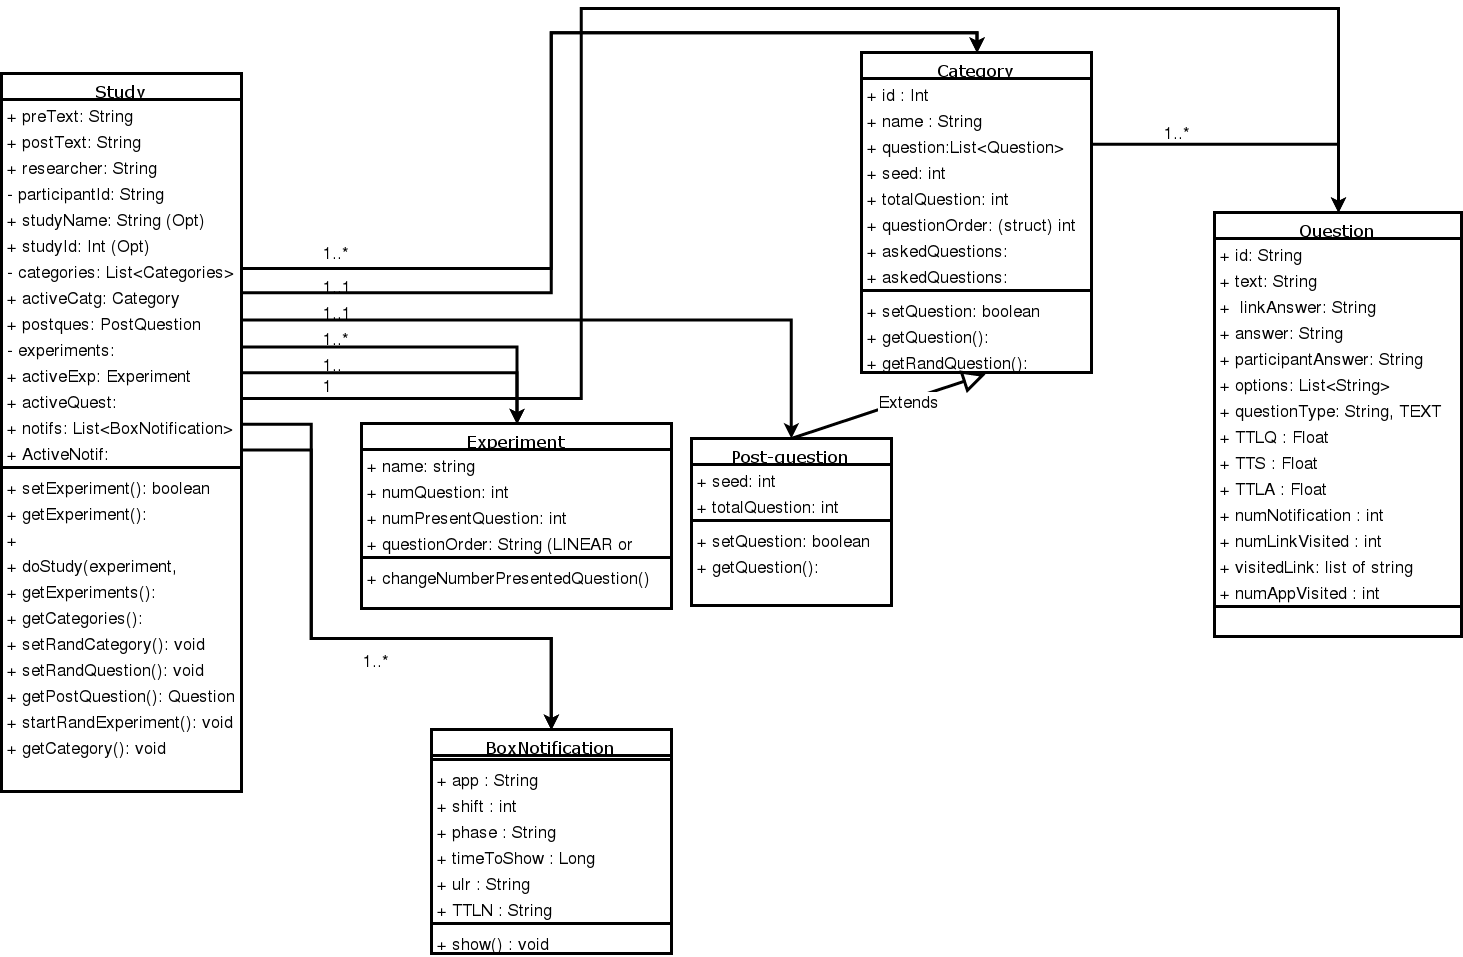
\includegraphics[scale=0.3]{class_diagram}
\end{center}
\caption{Class diagram}
\label{fig:class_diagram}
\end{figure}

\subsection{Study Class}
Study class is the class that act as a main container for other entities of the application and it control the flow of the main function of the experiment.
% The more description of the class variable including it's value and function can be seen on the table XX below. How the variable is set will be explained in this part.
Some of its properties are defined from input file: \textit{preText, postText, researcher, studyName, studyId}.
As seen in the class diagram \ref{fig:class_diagram}, the study class contains \textit{experiments} variable which consist of list of experiment objects
, \textit{categories} variable which consist of list of category objects and \textit{notifs} variable that consist of list of notification objects.

As explained in the design section, the experiment application need to initialize several variables before conducting the experiment. These variables define which experiment to conduct, which questions to show and which category to use. \textit{ActiveExp} (active experiment) present which experiment is conducted. this variable set by the researcher on the application. And \textit{ActiveQuest} (active question) present several  questions being asked to the participant the value of \textit{ActiveQuest} variable can consist of several questions object which will be shown during the quiz experiment. The question inside \textit{activeQuest} is picked from the list of question inside the active category (\textit{activeCatg}) variable. The \textit{activeCatg} variable is chosen by the participant during the experiment.


%After the category (\textit{activeCatg}) and set the experiment %(\textit{activeExp}) are chosen, the experiment can be started. The experiment will present the participant with one or several questions. In the study class there is \textit{activeQuest} (active question) variable that contains the  question objects that is being on a \textit{shift}.

Moreover, the class also contains the active notification (\textit{activeNotif}) this variable contains a list of notification that has been shown up to the participant. the notification come from the \textit{notifications} variable that contains list of notifcations.  the mechanism of the notification will be explained much further on the section \textbf{XX}.
\todo[inline]{mention which section is the notification}

% \begin{table}[!b]
%   \centering
%   \begin{longtable}{ |p{0.5cm}|p{4cm}|p{2.3cm}|p{6cm}|  }
%  \hline
%  No& Variable's name & Type & Description \\
%  \hline
%  1 & preText & string  & the text\\
%  2 & postText & string & THIS DESCRIPTION NEED TO BE FILLED\\
%  3 & researcher & string & True if the participant decide to look at the question again, false otherwise. \\
%  4 & studyName & string & total time (in millisecond) when the participant see the answer links and decide to look the question again or answer the question (next button) \\
%  5 & studyId & string & Similar with TTLB and the participant decide to look at the question again.Then, answer links are shown again to the participant\\
%  6 & participantId & List of String & The list of links clicked/visited by the participant after clicking the answer links\\
%  7 & randomGenerator & List of Long  & List of the total time (in millisecond) the participant stay on a page after clicking link\\
%  8 & categories & List of String & similar with visited\_links but the participant have decided to see the question again then return to the answer links window\\
%  9 & experiments & List of Long & Similar with time\_visited\_links but the participant decide to look at the question again then click the answer links\\
%  10 & postques & Long & Total time (in millisecond) the participant see the fill answer window and then click next\\
%  11 & activeExp & Long & Total time (in milisecond) the participant write the answer on the text box\\
%  12 &  activeCatg & Integer & how many notification is shown during the a question \\
%  14 & activeQuest & Long & Total time (in millisecond) it tooks the participant after clicking the notification to back to experiment application\\
%  15 & notifs & Long & Total time (in millisecond) it tooks the participant after clicking the notification to back to experiment application\\
%  16 & activeNotif & Long & Total time (in millisecond) it tooks the participant after clicking the notification to back to experiment application\\
%  16 & shiftNum & Long & Total time (in millisecond) it tooks the participant after clicking the notification to back to experiment application\\

% \hline
% \end{longtable}
% \caption{Variable inside study class}
%  \label{tab:studyClassVariable}
% \end{table} \par

The study class contains methods that is used to control the main flow of the experiment.
These methods will be explained on the next chapter.
\todo[inline]{which chapter explained the experiment}
\subsection{Experiment Class}
The Experiment class contains the \textit{\textbf{experiment properties}} that is used to define the behavior of the conducted experiment. The properties is explained more detailed in the table \ref{tab:ExperimentClassVariable}.

Every variables inside this class except \textit{numPresentedQuestion} is determined from the input file. It is has one method \textbf{changeNumberPresentedQuestion()} which is called by the study class to change the \textit{numPresentedQuestion} variable. The method will change the number presented question randomly from 1 to \textit{maxPresentedQuestion} by using using the Random object (RandomGenerator) provided by java.


\todo[inline]{snapshot of the code}

\begin{table}[!htb]
  \centering
\begin{longtable}{ |p{0.5cm}|p{4cm}|p{2.3cm}|p{6cm}|  }
 \hline
 No& Variable's name & Type & Description \\
 \hline
 1 & name & string  & The name of the experiment\\
 2 & numQuestion & Integer & The number of questions will be asked on the experiment \\
 3 & numPresentedQuestion & Integer & the number of question presented to the participant on the experiment every phase of question-answer \\
 4 & questionOrder & String & if the value is RANDOM, then the question is picked randomly from a list of question, if the value is LINEAR then the question will be picked based on the order of the input file \\
 5 & randomPresentedQuestion & Boolean & if it the value is true, then on each phase the num of presented question will changed randomly, explained more on changeNumberPresentedQuestion method \\
 6 & maxPresentedQuestion & Integer & this is the maximum number of presented question if the number of presented question is decided randomly\\
 7 & randomGenerator & Random  & this is a random class that use to generate random nunmber, it is used inside changeNumberPresentedQuestion method \\
\hline
\end{longtable} \par
\caption{Experiment class variables}
 \label{tab:ExperimentClassVariable}
\end{table}

\subsection{Category Class}
Category class is used to carry the questions objects that has the same category. The two main part of the variable are \textit{questions} and \textit{askedQuestion}. \textit{questions} variable simply is a list of questions, and the \textit{askedQuestion} is list of question that has been asked to the participant.

The class has two main methods \textit{getRandQuestion()} and \textit{getQuestion()}. These methods will be called during the quiz activity to put question object into activeQuestion variable.
These method aretwo different procedure to pick a question from list of question object inside \textit{questions} variable. the former take the random randomly while the latter will take the question based on the input order. After the question is selected, it will get deleted from the \textit{questions} variable and thenput it into \textit{askedQuestion} variable.
The \textit{getQuestion()} method get the latest question from the \textit{questions} variable which is similar to the input order. On the other hand \textit{getRandQuestion()} use the Random class the get the random index of the question.

\subsection{Question Class}
The Question hold the questions, it's answer and the tracked variable that is tracked when the question is being asked. The variables is explained more on the table \ref{tab:questionClassVariable}
, and the rest of the variable is explained on the tacked variable on the section XX.
\todo[inline]{what question to answer}
The question can be two type MC or TEXT. MC means multiple choice, this question type will have multiple options on it's answer, and the participant can chose one of them. while TEXT means that the participant need to write the question.

\begin{table}
  \centering
  \begin{longtable}{ |p{0.5cm}|p{4cm}|p{2.3cm}|p{6cm}|  }
 \hline
 No& Variable's name & Type & Description \\
 \hline
 1 & id & string  & the id of the question\\
 2 & text & string & the text of the question\\
 3 & linkAnswer & string & the URL link to the answer page \\
 4 & answer & string & (optional) the answer of the question \\
 5 & participantAnswer & string & the answer of the participant during the quiz activity\\
 6 & questionType & String & The type of the question, the value can be "MC" or "TEXT".\\
 7 & representId & string  & present id shows if two or more questions are presented together during quiz activity\\
 7 & options & list of String  & List of the total time (in millisecond) the participant stay on a page after clicking link\\
\hline
\end{longtable}
\caption{Variable inside Question class}
 \label{tab:questionClassVariable}
\end{table} \par


\todo[inline]{where to get the traccked variabel}

\subsection{BoxNotification class}
BoxNotification class present the Notification. BoxNotification is used as a class name because Notification is already defined class.
The variable inside the class is explained on the table X.

The Notification can open an android application of twitter, facebook, instagram and web browser. The application should be installed to the phone, otherwise the notification will open the url of the application on the web browser.
This app need to be specified on the \textit{app} variable and the \textit{url} variable. The \textit{url} variable need to be filled with the user id of the twitter or instagram. Or it can be filled with http/https url to open web page. the class contains a show() method that will pop up the notification in the android phone.
The the mechanism and flow of the notification will be explained on chapter XX


\todo[inline]{where is the notification flow}


\begin{table}
  \centering
\begin{longtable}{ |p{0.5cm}|p{4cm}|p{2.3cm}|p{6cm}|  }
 \hline
 No& Variable's name & Type & Description \\
 \hline
 1 & app & string  & The application that can be opened by the notification \\\
 2 & shift & Integer & The number of questions will be asked on the experiment \\
 3 & phase & Integer & the number of question presented to the participant on the experiment every phase of question-answer \\
 4 & timeToShow & String & if the value is RANDOM, then the question is picked randomly from a list of question, if the value is LINEAR then the question will be picked based on the order of the input file \\
 5 & url & Boolean & if it the value is true, then on each phase the num of presented question will changed randomly, explained more on changeNumberPresentedQuestion method \\
 6 & titleText & Integer & this is the maximum number of presented question if the number of presented question is decided randomly\\
 7 & msgText & Random  & this is a random class that use to generate random nunmber, it is used inside changeNumberPresentedQuestion method \\
\hline
 8 & presentedID & Random  & this is a random class that use to generate random nunmber, it is used inside changeNumberPresentedQuestion method\\
\hline
\end{longtable}
\caption{Variable inside Question class}
 \label{tab:questionClassVariable}
\end{table}

\section{Application flow}
In this section the flow of the application on the technical aspect will be discussed.
The flow of the application can be seen
on the figure \ref{fig:flowApp}. The application is divided into four scope.
\begin{itemize}
\item Setting study : this part the researcher can set the properties of the experiment and choose to start the experiment.
\item Experiment : this part when the participant conduct the experiment.
\item Notification : this part when the notification can be shown up on the activities.
\item PostQuestion : this part when the participant presented with post questions.
\end{itemize}


\todo[inline]{Need to write more about the bullshit here}

Each class activity and method on the flow chart is explained further on the subsection

\subsection{Android Activity}
The android application built upon multiple class activities. Each activities has an user Interface (UI) template. the UI consist of button, text, etc. And its corresponding class activity will decide what will appeared on the phone or what happen if a button is clicked . The event such us clicked or move to another application can be detected and linked to an \textit{event listener} methods which will get called every time the event happened.

Figure \ref{fig:theLifeCycleOfActivity} show how the android activity lifecycle. There are three main activities method used in this experiment application. \textit{OnCreate()} is the first method to get called everytime the activity start. \textit{OnPause()} will be called if the user of the phone move / redirected to another application. Lastly,  \textit{OnResume()} is called if the user open the application again after leave the application.



\begin{figure}[!b]
\begin{center}
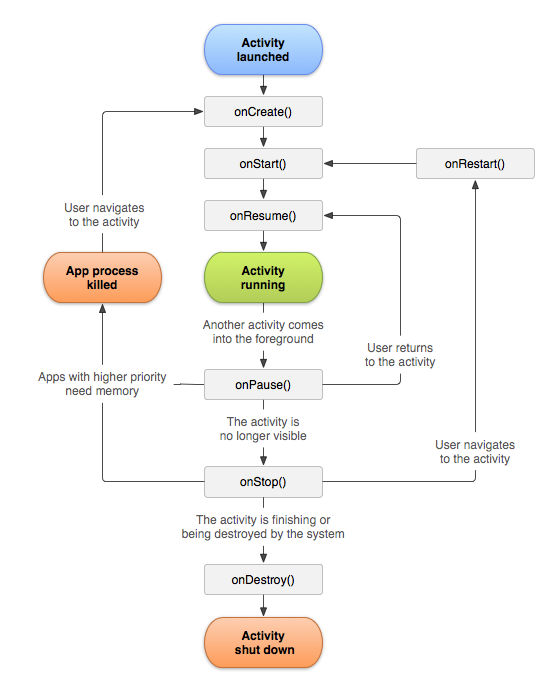
\includegraphics[scale=0.3]{activityLifeCycle}
\end{center}
\caption{The cycle of activity}
\label{fig:theLifeCycleOfActivity}
\end{figure}



\subsection{expInitialActivity}
The UI layout of these activity can be seen in figure \ref{fig:expInitActLay}. The participant can click a button to begin the experiment or to set the properties of the experiment.

On the OnCreate() event listener of the activity the InputReader.read() method is called. This method will read the input data and compiled it into Study object. The input  data as string is compiled into json object by using gson library. Gson is a serialization / deserialization library that is used to convert string of object into json or another way around.


After reading the input file and compiled into The \textit{Study} object. the object is need to be sent from an activity to another activity. \textit{Intent} class of java is used to encapsulate the object and send to another activity. Because the \textit{Study} object need to be encapsulated inside the Intent, java programming language require class of the object should implement the Serializable class.


\todo[inline]{snapshot of the intent code}


\begin{figure*}
\centering
\begin{minipage}[b]{.4\textwidth}
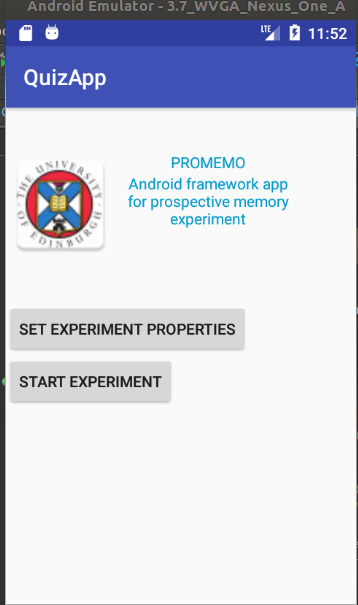
\includegraphics[scale=0.32]{FE_1}
\caption{Caption}\label{label-a}
\end{minipage}\qquad
\begin{minipage}[b]{.4\textwidth}
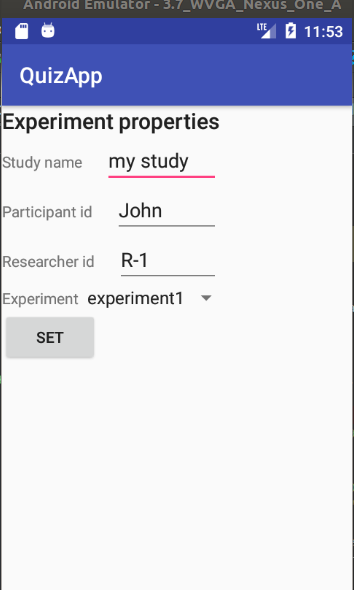
\includegraphics[scale=0.32]{FE_set_properties}
\caption{Caption}\label{label-b}
\end{minipage}
\end{figure*}

\subsection{expSetPropActivity}
This activity is used to set some parameter of the experiment. In this activity the researcher can pick which experiment to conduct and change the participant name. The purpose of this activity is to make it easier for the researcher to conduct multiple experiment and multiple participants without uploading the input file again. Figure XX shows the

\todo[inline]{Do I need a snapshot of code here?}
\subsection{IntroActivity}
This activity is used to show the information about the experiment to the participant before starting the experiment. These information is stored inside the preText and postText string. the value of this variable will be converted into html and shown respectively.
Figure X show example of the Consent information shown inside the application.

\subsection{ChooseCategoryActivity}
In this activity the participant choose which category he/she want to answer, as seen in the figure XX.
\todo[inline]{Also do I need to attach my code here?}
Radio button represent the options of the category in the UI class. the selected category name will then save in the selectedCategoryName variable inside study class as seen in the code XX.

\subsection{QuestionActivity}

In this activity, the question inside activeQuestion variables are shown to the participant. This activity will be called multiple time during the quiz experiment.
the activity mainly call Study.runExperiment() method on the OnCreate() event. this method is the main method of the experiment, it use to start or continue the quiz experiment. this method is explained on the section below.

\subsubsection{Study.RunExperiment()}
This method will be called everytime in the beginning of the Quiz activity.
The main function of this methods are :
\begin{itemize}
\item Initialize the active experiment (\textit{activeExp} variable) and active category (\textit{activeCatg}) variable.
\item Change the number of \textit{presentedQuestion}, the variable is explained in the Experiment class.
\item Set the active questions (\textit{activeQuest}) from the questions in the category.
\end{itemize}

Figure \ref{fig:RunExpflowApp} show the flowchart of the method. The First step is to initialize the experiment by checking the active experiment (activeExp) variable. if it's empty than it's mean that this is the first time the experiment run and it needs to initialize.
Two main experiment properties which are active experiment (activeExp) and active category (activeCatg) are initialized by calling \textbf{initializeExperiment} method. The \textbf{initializeExperiment} method will initialize the experiment based on the \textit{selectedExperimentName} and \textit{selectedCategoryName}.


the \textbf{setRandomPresentedQuestion()} is called, this method will set the value of numPresentedQuestion which is the number of question presented on each phase of question-answer quiz. If the resercher set randomPresentedQuestion to true in the input file, then the value of number of presented variable will be random in the range of 1 to MaxPresentedQuestion. On the other hand if it's false, then the numPresentedQuestion will be constant.

Next, \textbf{isExperimentIsStillGoing()} is called. This method make sure if the experiment is still in on on going by checking that if the size of the \textit{question} variable inside the activeCatg is still larger or similar to \textit{numPresentedQuestion}. so it's still possible to pick the question form the \textit{questions} variable.

Lastly, the active question (\textit{activeQuest}) is picked from the questions variable by calling \textbf{setActiveQuestion()}. this method will pick and put the question object from activeCatg into the  \textit{activeQuest} variable. the question object will be picked randmly if the researcher set questionOrder to random, otherwise the question will be pick linearly.


\subsubsection{AnswerActivity}
In this activity the answer link are shown as a textview inside the UI layout. If the participant click the answer link then the clickListener inside the textview will open an answer window. An java class called \textit{webview} is used as a browser of the answer page based on the URL of the answer link (question.url).

Two radio buttons are presented to the participant. These are the option whether the participant want to go back to see the question again or to continue to answer the question.

If the participant chose back then the application will go to question activity. on this transition the string is also capsulated inside the intent along with the study object. this string called "BACK" is used as a flag. This flag is send to question activity and send back to answer activity. this flag is used to know if the participant look at the question again.
If the back flag is present on the answerActivity then the radio button to see the question again is hidden by setting it's visibility to GONE, as it seen on the snapshot of the code.
\todo[inline]{put the snapshot of the code}

\subsection{fillAnswerActivity}
In this activity the participant should answer the question by writing the answer on the editText UI as seen on figure.

each editText is correspond with one question presented before, there can be multiple editText because there can be multipe question.

If the participant click next button then saveAnswer() method is called which will get the value of the editText and stored it on the participantAnswer on activeQuest.



\begin{figure}
\begin{center}
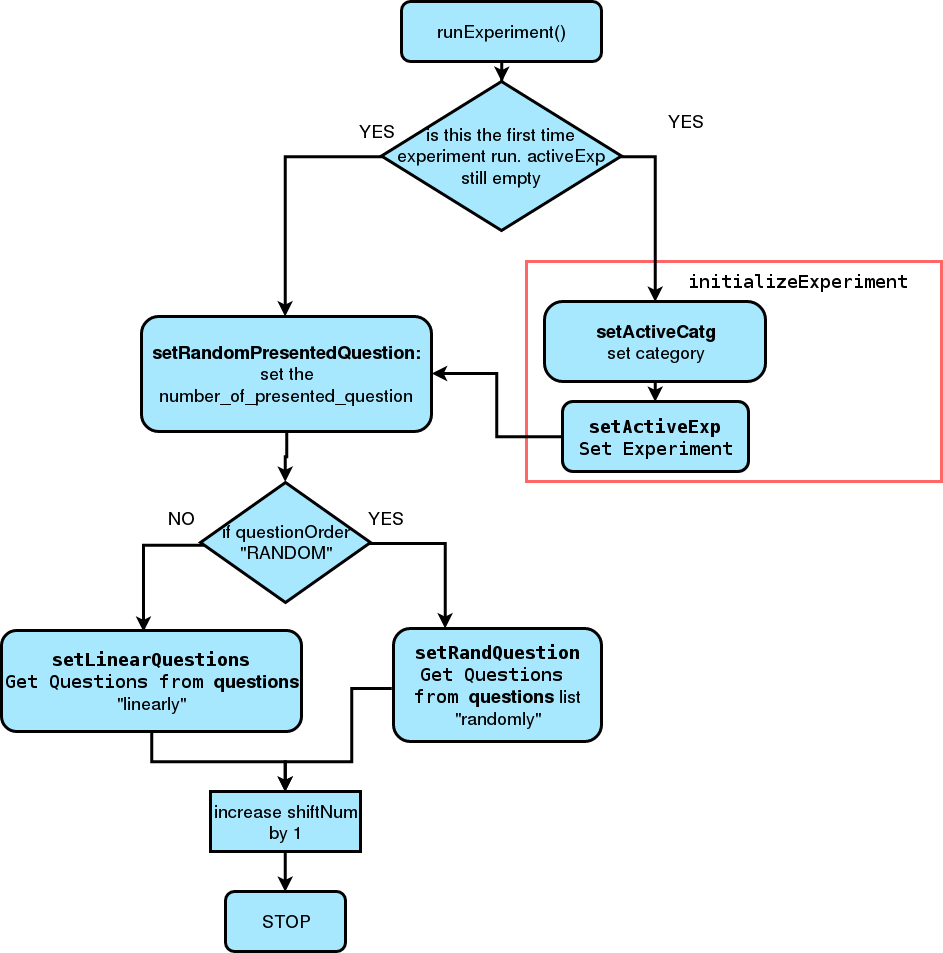
\includegraphics[scale=0.5]{runExperiment}
\end{center}
\caption{runExperiment flow chart}
\label{fig:runExperiment_flow}
\end{figure}


\begin{figure}
\begin{center}
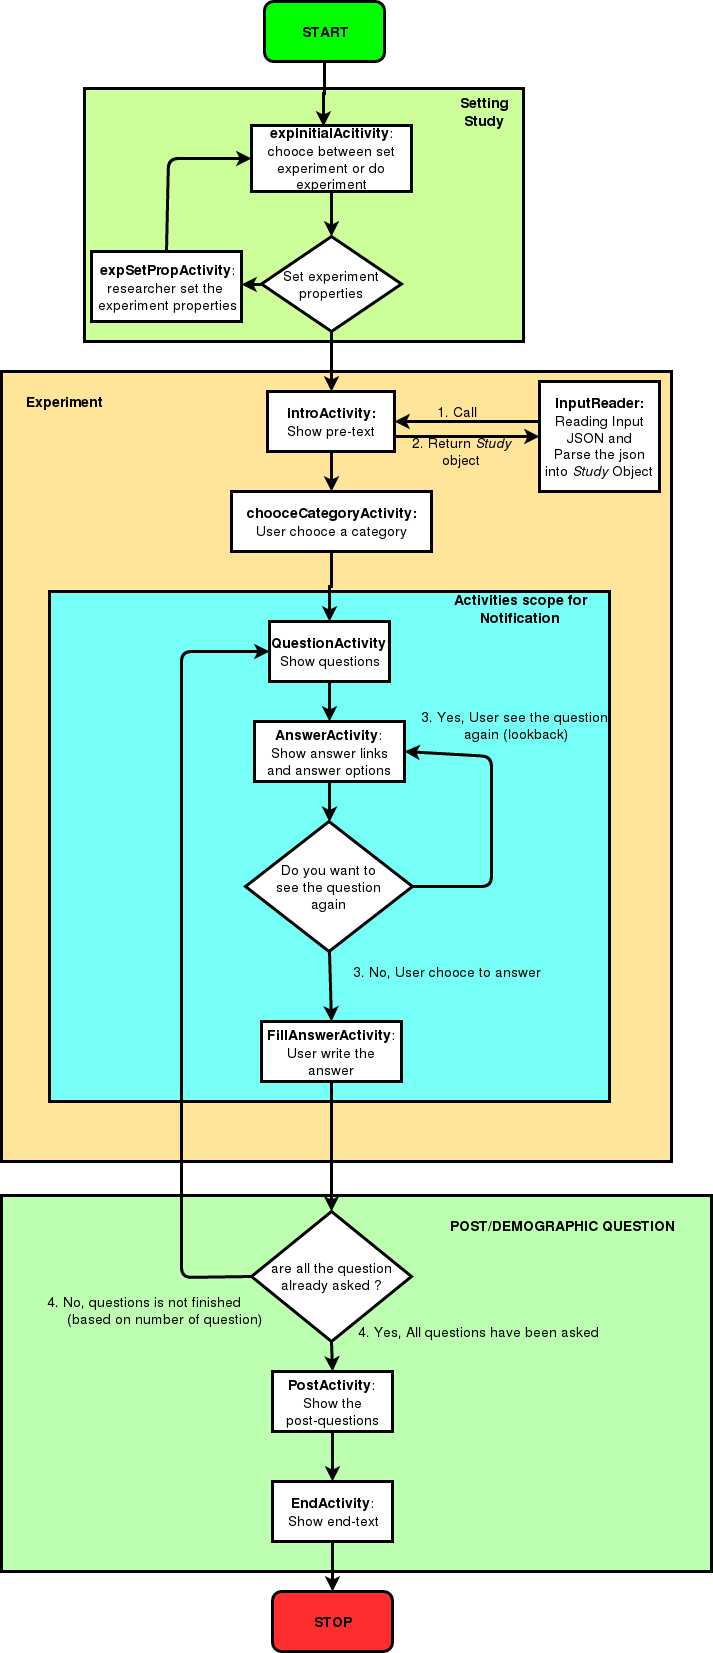
\includegraphics[scale=0.35]{Flowchart_}
\end{center}
\caption{The flow of the application}
\label{fig:RunExpflowApp}
\end{figure}

\section{Notification mechanism}
Figure \ref{fig:NotificationFlo} shows the mechanism of notification.
As seen on the flowchart, the Study.checkNotification() method is called inside the OnCreate event on the QuestionActivity, AnswerActivity and FillAnswerActivity. The method check on every notifications inside the \textit{notifs} variable if the there is a notification that should be shown up based on phase and shift variable of the notifiaction. these variable is comapred with the variable passed by the method.

If there  is a notification that need to be shown up then the notification object is added into the activeNotif and it is deleted from the notifs variable of the study object.

The notification need to wait for some millisecond before it can be shown up. The waiting time is defined in \textit{timeToshow} variable inside the BoxNotification class.
While the notification process wait, the main activity (Quiz) should keep working so another process need to be made a part from the main process. To accomplish it, TimerService class is used. This class will be spawn as another process and the process will be sleep for \textit{timeToShow} millisecond then it will call the broadcastReceiver method which is defined inside each activity.
This method will called  the show method inside the notification.

The \textbf{Notifaction.show()} method is used to shown the notification to the front end of the android screen. This methode use
 NotificationCompact.Builder is used To build the notification layout. an Intent object is inserted inside the Builder object that contains what application to open. If the participant click the notification then the experiment application will be minimized. this event will call OnPause() methode on the current activity, and the android phone will open the intended application. The participant can go back to the current app by opening the application again and the OnResume() method  of the current activity is called.


\section{Tracker}

The tracked variable are shown on the table \ref{tab:trackedVarible}. All of these variable are stored inside the Question class as it seen in the class diagram \ref{fig:class_diagram}.

Some of the variables use to track the time in millisecond. To track the time the StopWatch class provided by java API is used. The StopWatch object is stored inside the study class because the StopWatch class is not serizable which means it can not be pass in the Intent object inside the Study class.

During the experiment the application will be minimized if the participant click the notification. During this event some Stopwatch object need to be pause. the OnPause() method of the curent activity is called when the application is minimized which is used to suspend the stopWatch and it will be resume again after OnResume().


\todo[inline]{this need to be explained}

As it seen in the class diagram, each one of tracked variable has it's own StopWatch object for example StoWatchTTLQ will track the time for TTLQ variable. to stored the time tracked by the stopwatch the Study.log() method is called. this method pass two arguments, what variable to track and the stopwatch object used to track it. for instance log("TTLQ",stopWatchTTLQ) will track the TTLQ variable inside the activeQuest and use stopWatchTTLQ to get the tracked time.
How each variable is tracked is explained further on the subsection below.

\subsubsection{TTLQ, lb\_TTLQ and lookback}
These variable is tracked inside the QuestionActivity. StopWatchTTLQ and stopWatchTTLQ\_lb is used to track the timing of this variable. The stopwatch object start to count the time when OnCreate() method is called on the current activity, and the stopwatch will be stopped when the participant click next button. The Study.log() method will be called to track the variable when the next button is clicked. Inside the Study.log() method, it will call logTTLQ or logTTLQ\_lb methods to stored the value of the tracked variable on each question object inside the activeQuest. the stopwatch variable will be passed on these method and the milisecond didapat bycalling StopWatch.getTime() method.
The lookback variable will have true value if the participant chose to see the question again. These variable is set on the logTTLQ\_lb() method.

\subsection{TTLB and lb\_TTLB}
These variable are tracked inside the AnswerActivity. Similar with TTLQ, stopwatchTTLB and stopWatchTTLB\_lb is used to track these variable. The stopwatch will start on Oncreate() method and it will be tracked when the participant click the next button.

\subsection{visitedLinks, lb\_visitedLinks, timeVisitedLinks\\ and lb\_timeVisitedLinks}
These variable is tracked inside the AnswerActivity.

During the AnswerActivity if the participant click the answer link then the \textit{webview} class of java is used to open the URL link. StopWatchLink then will be started, and it is used to track the time participant have spent on each web page inside the webview.

The mechanism of the tracking is shown in the figure \ref{fig:webViewTrack}. Firstly, the prevUrl variable is initialized, this variable stored the previous link the webview had opened. This webview class has an event listener called onPageFinished() which will called every time the web page has been finish loaded for example when the participant click the answer link or visit another link on the webpage. Every time the event listener onPageFinished() is called, or when the participant click the button then updateVisitedLinks() method is called. updateVisitedLinks() method stored the value of prevUrl (because it has been visited before) to visitedLinks variable and how long the participant spent on the web page to timeVisitedLinks.
\todo[inline]{check again}

\subsection{TTLA and TTLFA}
These variable are tracked on the fillAnswerActivty. the TTLA simply tracked similar to TTLQ and TTLB, the variable tracked using StopWatchTTLA.

TTLFA is tracked differently because if there is more than one question then there will be multiple editText for the answer field.

On each editText element, the event listener called OnFocusChangeListener is attached to it. this event listener will be called if the is a change of focus on the UI layout of the activity, for example if the user click one editText then click another one. the event listener method can give an UI id of which editText was the user writing on before moving to another editText. the UI id will be stored inside the activeViewId variable.

{should I attach some code}. After getting the UI id a stopwatch corresponding on the editText should be obtained to track the time.
To accomplish this stopWatchTTLFA is made as a hashmap where the key is the UI id, the id is made from the index of the question inside the activeQuest variable, and the value is the stopwatch correspond to the editText answer. so to access which Stopwach object correspond to particular editText the UI id from the event listener will be used to get the corresponding stopwatch object.

to track the time updateTTLFA() method is called this method will track the TTLFA time by accessing the stopwatchTTLFA hash map using the activeViewId variable.

\todo[inline]{jesus is hard to explain this}

\subsection{numNotif, numNotifClicked and TTLN}
As explained on the section 4.3.8 during the QuestionActivity, AnswerActivity and fillAnswerActivity the checkNotifaction() will find the notification that should be shown up to the screen and it will called the inceraseNumNotif() method.
This method will increase the numNotif variable of every question inside activeQuest.

If the notifaction is clicked then the inceraseNumNotifisClicked() method will be called inside the broadCastReceiver on the current activity class. This method will increase the number of numNotifClicked variable on every question object inside the activeQuest variable.

notifStopWatch object is used to track the TTLN time. After the participant click the notification than the application will be minimized and other application will be opened. As explained on the Android activity section (4.3.1), the OnPause() event handler will be called just before the application is minimized. On OnPause() method a Study.startLogNotif() method is called, this method will start the notifStopWatch object.
Then after the participant got back to the experiment application the onResume() method is called. This method will call Study.stopLogNotif() method. This method will get the current notification and set the TTLN from the notifStopWatch.
\cite{Kliegel1984}

%\todo[inline]{WHAT THE FUCK TO WRITE}

\begin{figure}
\begin{center}
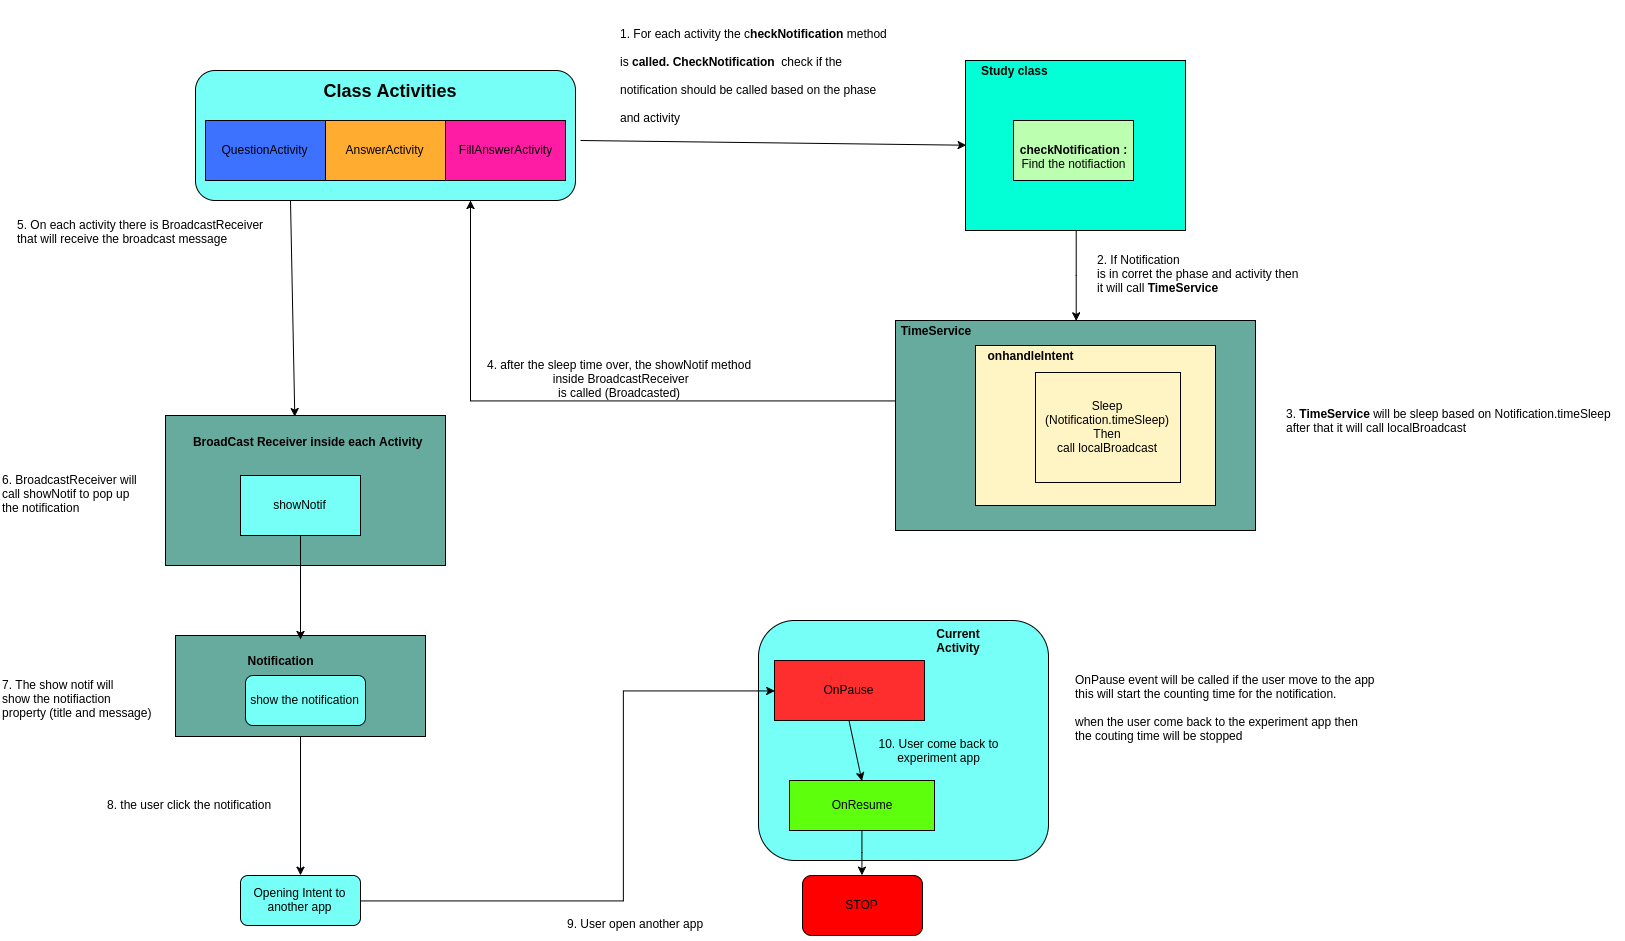
\includegraphics[scale=0.35]{notification_diagram}
\end{center}
\caption{The flow of the notification}
\label{fig:NotificationFlo}
\end{figure}
\todo[inline]{increase the font}

\begin{figure}
\begin{center}
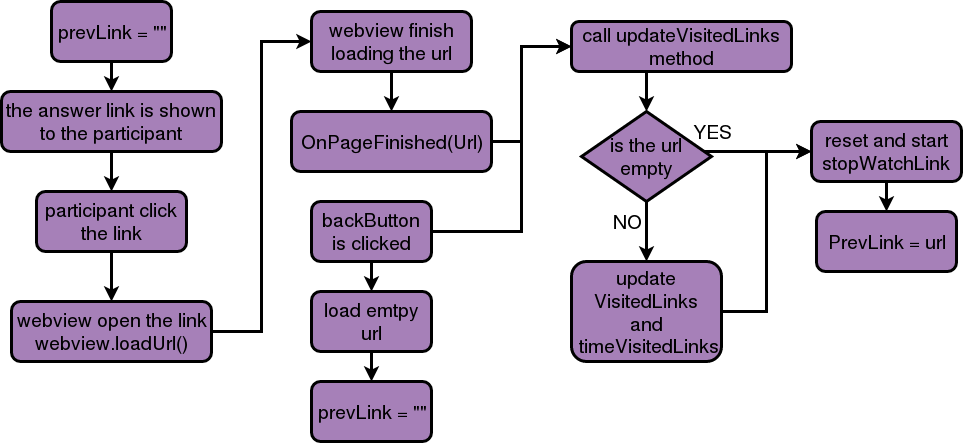
\includegraphics[scale=0.5]{tracker_linkVisited}
\end{center}
\caption{tracker mechanism for webview}
\label{fig:webViewTrack}
\end{figure}
